The presented papers all had the goal to research the possibilities to use the parallel performance of the GPU for video encoding. 
\todo{The, typo I suppose should be they} conducted different experiments for speed-up and RD-Performance (quality of the encoded video). 
In this section their experimental set-ups and their results are shown and compared.\\
\\
In the first paper \cite{Paper1} the authors conducted experiments on a PC equipped with one GeForce 8800 GTS PCIe graphics card with 96 stream processors \cite{geforce8800}, 
and an Intel Core 2 Quad Q9400 2.66 GHz CPU with 3.23 GB of RAM. To implement the GPU code, they used NVIDIA's Compute Unified Device Architecture (CUDA) \cite{nvidia2programming}. \\
They conducted multiple experiments with their implemented code on CPU+GPU, where the fast ME was executed on the GPU and compared their results to the JM 14.2 reference software on a single core and on a quad core. 
They used the H.264 high profile with a search range of 64. The chosen tile height was always \textit{L=1}. The video sequences were at HD 720p(1280x720 pixels, 60 frames per second).\\
The result of the quad core comparison is depicted below in figure \ref{tiling_speedup_mc}.
\begin{figure}[H]
\centerline{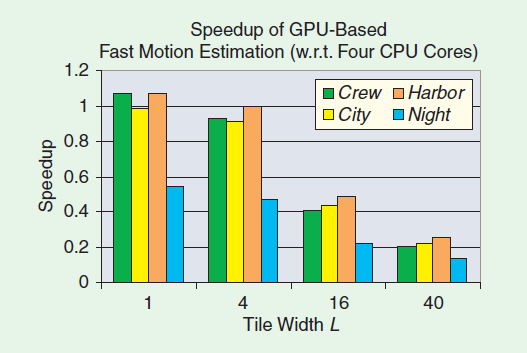
\includegraphics[scale=0.4]{pics/tiling_speedup_mc}} % The bounding box is set manually in this example. Useful for some .pdf figures.
\caption{\label{tiling_speedup_mc}{
\it Trade-off between tile width and speed-up (taken from \cite{Paper1})
%\footref{ftn:speedup} (tile height \textit{K} is
%equal to one) TODO
.
}}
\end{figure} 

The experiments on the speed-up indicate that with their tiling approach they reach a minimal speed-up of around 5\% for certain sequences like \textit{Crew} and \textit{Harbor} at a tile width of \textit{L}=1. 
In every other constellation of tile widths the quad core CPU is equally fast or mostly faster than their implementation.\\

\todo{put following sentences into one paragraph make more sense}
As for the evaluation of the RD performance the results showed the average peak signal-to-noise-ration (PSNR) degradation and the average increase in bit rate using different tile sizes, 
measured by Bjontegaard Delta PSNR (BDPSNR) and Bjontegaard Dekta bit rate (BDBR)\footnote{BDPSNR and BDBR are used frequently in the video standardization community \cite{bjontegaard}} respectively.
The results suggest tiling may lead to average degradation between 0.08 dB to 0.4 dB for these sequences with a tile size of \textit{K}=1, \textit{L}=1.
Their loss in quality is of course due to the loss of information on MVs. \\

A possible explanation for the low speed-up might be the access latency of the memory. 
Their encoder is implemented to store the pixel data needed by the GPU in the off-chip memory which generates high access latencies. 
A possible solution would be to use memory coalescing, which means that all the threads would read from the memory at the same time from one memory bank. 
\todo{no, this is not memory coalescing, thread in warp(a group of threads) access consecutive elements stored in memory, they are not in the same one memory bank}
\todo {Thus the frame data has to be sequential inside the memory, I don't get it}, but it would speed-up the memory access enormously.
\todo {another tip here is that with configuration K=1 L=1, maximum number of threads can be launched for one frame, therefore more parallelism can be exploited}\\

The second paper \cite{Paper2} also used the JM encoder as reference software, but in version 17.2. They ran their experiments on PCs with an Intel Core i/ with 3Ghz and an Intel Core 2 Quad with 2 Ghz. Both Platforms have 4GB memory and use a Geforce GTX 580. The results presented here are regarding the Core 2 Quad, to better compare it with the other papers.\\
The video sequences used were at 1080p (1920x1080) and they chose a search range of 32.\\
Their implementation of the dynamic distribution model was compared to the following:\\
\begin{itemize}
\item \textbf{CPU-only}: the whole encoder is implemented in the CPU
\item \textbf{GPU-only}: the whole encoder is implemented in the GPU
\item \textbf{Chen\_original}: method proposed by Chen \cite{chen2008h}, where the ME, SME and
interpolation modules are statically offloaded to the GPU
(the rest are kept in the CPU)
\item \textbf{Chen\_optimized}: Chen's encoder \cite{chen2008h}, optimized with \\OpenMP and SSE4 vec-
torization techniques
\item  \todo{\textbf{Proposed}: presented dynamic load distribution strategy, why their implementation would compare to the proposed, I think this one should be removed}
\end{itemize}
The author didn't clearly specify the GPU-only implementation and  what it specifically means for the different parts of the algorithm and is therefore ignored in this article.\\
In figure \ref{dynamic_model_result} the results of the experiment is shown.

\begin{figure}[H]
\centerline{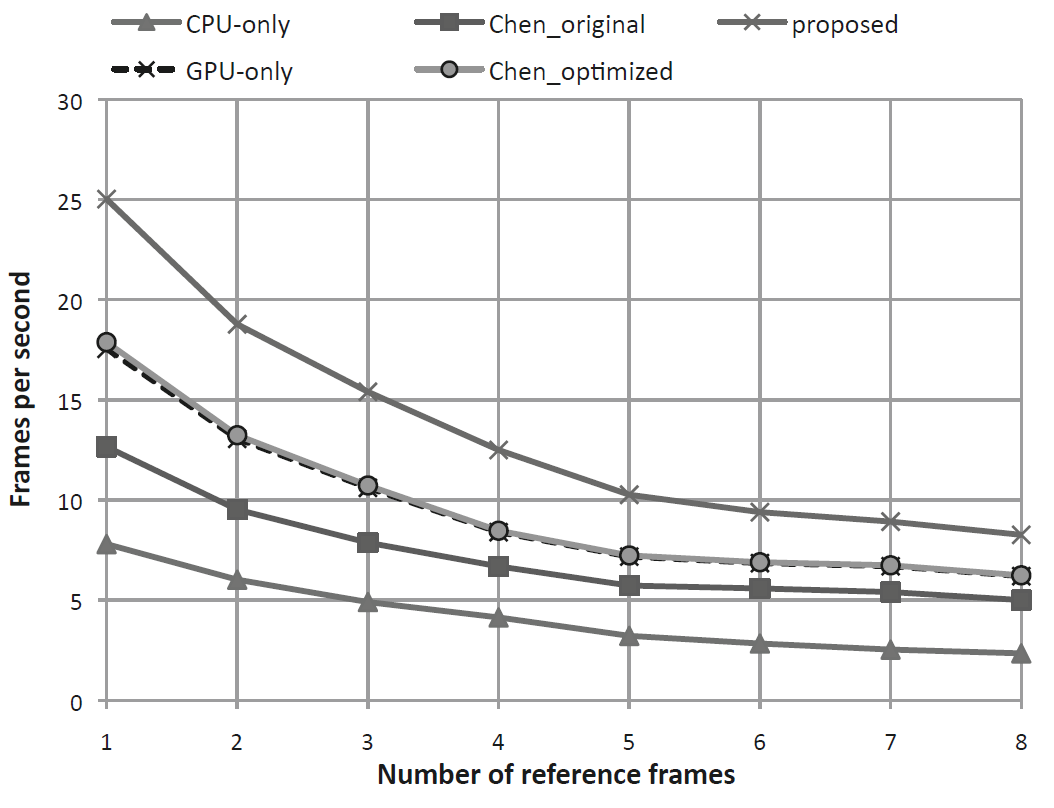
\includegraphics[scale=0.3]{pics/dynamic_model_result}} % The bounding box is set manually in this example. Useful for some .pdf figures.
\caption{\label{dynamic_model_result}{\it Encoded frames per second (fps)
 for a varying number of RFs, using the 1920x1080  video format.
  Comparison of the proposed approach with CPU-only, GPU-only and the
  approach proposed by Chen (taken from \cite{Paper2}).}}
\end{figure}

The proposed method reaches a speed-up of around 25\% compared to the Chen optimized encoder, around 500\% compared to the CPU only, respectively. Besides the increased performance of the proposed dynamic distribution model, the approach of the authors guarantees a certain independence from the adopted devices. In case either the CPU or the GPU is slow, the distribution model would have a different minimal path than with different devices. Of course the proposed method will only guarantee a speed-up if the distribution between the devices is useful. In case only the CPU is fast, there would be an immense overhead for the communication between CPU and GPU without any distribution to the GPU. 
Therefore it has to be taken into consideration, that the dynamic load distribution model is only of good use in specific cases of hardware configuration.\\
\\ 
The third paper \cite{Paper3} used the workstation Z620 from Hewlett-Packard with a NVIDIA Tesla C2050 GPU (448 CUDA cores at a clock rate of 1.15Ghz) for their experiments. The used CPU is not mentioned in the article.\\
They evaluated the acceleration performance of the improved VBSME on GPU and the RD in comparison to the reference encoder (HM9.0 \cite{hmencoder}). The proposed framework runs on CPU and GPU, \todo{typo seriell} and parallel. 
The reference encoder is only executed on a single CPU core. The search range is 64x64 with the full search strategy. They used two test video sequences with different
resolutions: \textit{BasketballDrive} (1920x1080 - 50fps) and
\textit{Traffic} (2560x1600 - crop).\\
Th results of their experiments regarding the speed-up are shown in table \ref{hevc_table_result}

\begin{table*}[ht]
  \centering
  \begin{tabular}{cccc}
    \textbf{Sequence} & \textbf{CPU(fps)} & \textbf{GPU(fps)} & \textbf{Speedup ratio in \%} \\
    Traffic\_2560x1600 & 0.21 & 23.77 & 113.2\\
    ParkScreen\_1920x1080 & 0.69 & 77.76 & 112.7\\
 \end{tabular}
 \caption{ \label{hevc_table_result}{\it Speedup gains on different video sequences (data taken from \cite{Paper3})}}
\end{table*}

The proposed CPU + GPU framework reached an immense speed-up of about 113 times the speed of the encoding time of the single core with the HM9.0 encoder. The authors reached an impressive result in their experiments but didn't quite take a width use of their setup into account. Full search is usually not used for ME because then the whole reference frame is scanned and therefore it takes a lot of time. They also compared their optimized results to the HM9.0 encoder which was executed on a single thread on a CPU not specified in the paper. The authors don't go into detail about any further optimizations for their framework or for the HM encoder and therefore it is possible that in a slightly different setup the speed-up would not be as big as in the experiments. \\
Another experiment they conducted was regarding the quality of the encoded video. Due to the fast decision mode they implemented they predicted some quality loss. In figure \ref{hevc_rd_result} the results are presented.\\

\begin{figure}[H]
\centerline{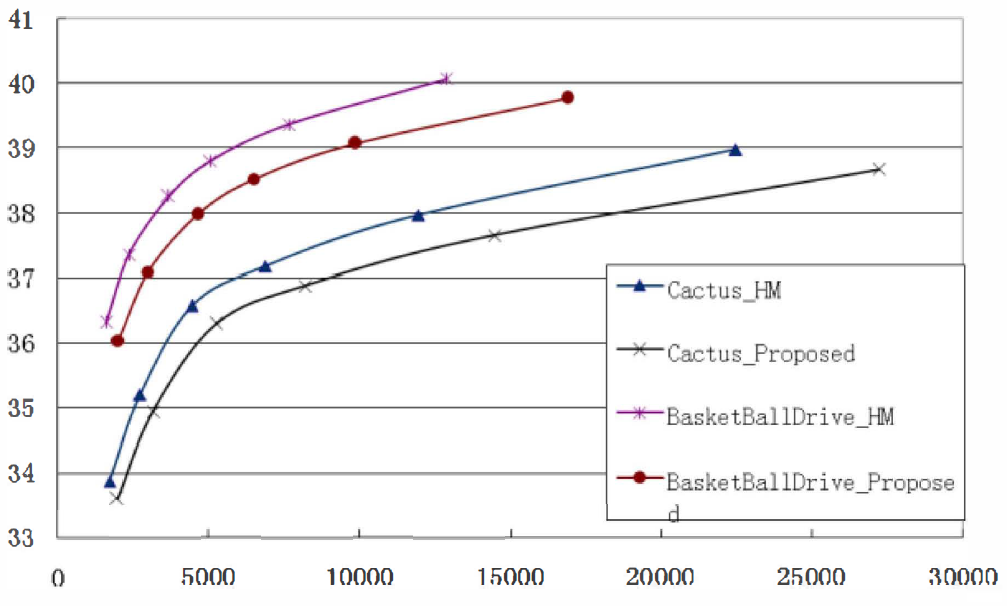
\includegraphics[scale=0.3]{pics/hevc_rd_result}} % The bounding box is set manually in this example. Useful for some .pdf figures.

\caption{\label{hevc_rd_result}{\it RD curve of the HM encoder and the proposed encoder. (taken from \cite{Paper3}}}
\end{figure}

The diagram shows the RD curves of the two encoders. From these RD curves, it can be seen that the RD performance degradation of the proposed
encoder with fast CU partition decision algorithm is about
0.7 dB degradation (calculated by BDPSNR \cite{bjontegaard}), which is a significant loss in quality.
\todo{you can criticize more, not only the DB, but also mention the degradation of bit rate, their solution increases 40\% more bit rate, which should be avoided.}\\
\\
The three papers all presented results regarding the use of the parallel performance of the GPU for certain tasks of the H.264 or H.265 codec.
Paper 1 is the only one that is using a fast ME algorithm\todo{are you sure the second paper also use full search? please check} and therefore no full search for their experiments. 
Full search is for real applications usually not an option and therefore not the best comparable setup.\\
Despite that the first paper didn't really reach a mentionable speed-up with even a great loss of quality. 
The experiments of the third paper show a similar result towards the quality (even worse) due to the fast decision mode. 
But in comparison to the first paper they reached a high speed-up, although the experimental setup is not enough specified. 
The second paper seems to be the most legit regarding the experimental setup and results. They compared they model to an optimized algorithm and specified the machines it was tested on. 
They also used \todo{are you sure the second paper also use full search? please check} a full search algorithm and reached a speed-up between 1.5 - 2 times which seems way more legit then the 113 times from the third paper. 